% class
\documentclass[a4paper,12pt,xelatex,ja=standard]{bxjsarticle}

% packages
%% mathematical notations
\usepackage{amsthm,amsmath,amssymb,amsfonts} % mathematical notations
\usepackage{bm} % bold character
\usepackage{latexsym} % more mathematical notations
\usepackage{physics} % physical notations
%% graphs
\usepackage{graphicx, xcolor} % graph
\usepackage{circuitikz} % for circuit elements
\usepackage{float} % positioning of graphs
\usepackage{siunitx} % SI units
\usepackage{tikz} % graphic elements
\usepackage{wrapfig} % must be after float package.
%% type system
\usepackage{bussproofs} % proof tree
%% code
\usepackage[ruled,vlined]{algorithm2e} % pseudo code
\usepackage{listings} % source code
\usepackage{inconsolata}
\lstset{
  basicstyle=\footnotesize,
  numbers=left,
  frame={tb}
}

% Basic information
\title{電子情報学専攻 \, 専門 \\ 平成21年 \, 解答・解説}
\author{diohabara}
\date{\today}

\begin{document}
\maketitle

\section*{第1問\ 電気・電子回路}

\section*{第2問\ 計算機アーキテクチャ}
\subsection*{(1)}
\subsubsection*{構造ハザード}
同じハードウェア資源を複数の命令が利用しようとすることによる、資源不足によるハザード

\subsubsection*{データハザード}
前の命令の結果をあとの命令が利用するフロー依存が存在する場合に生じるハザード

\subsubsection*{制御ハザード}
分岐命令がある場合に、その結果が確定するまで次の命令が決定できないために起こるハザード

\subsubsection*{ハザードと分岐予測の関係}
分岐予測によって、制御ハザードを解決できる場合がある。

\subsection*{(2)}
求めるサイクル数は以下のように表せる。
\[
  \frac{n \text{[instruction]}}{i_0 \text{[instruction / cycle]}} = \frac{n}{i_0}\text{[cycle]}
\]

\subsection*{(3)}
分岐予測ミスが0な、理想的なときに比べて、ペナルティ($\beta bnp$)サイクルだけ増加するので(2)より求めるサイクル数は
\[
  \frac{n}{i_0} + \beta b n p
\]

\subsection*{(4)}
プログラムの総実行命令数は変わらない。分岐予測ペナルティによってサイクル数が(3)の増えたのだから求める

\[
  i(\beta) = \frac{n}{\frac{n}{i_0} + \beta bnp} = \frac{i_0}{1 + \beta b p i_0}
\]

\subsection*{(5)}
数値を代入して
\[
  i(\beta) = \frac{2}{1 + 4 \beta}
\]

となる。グラフの外形は次の通り。

\begin{figure}[H]
  \centering
  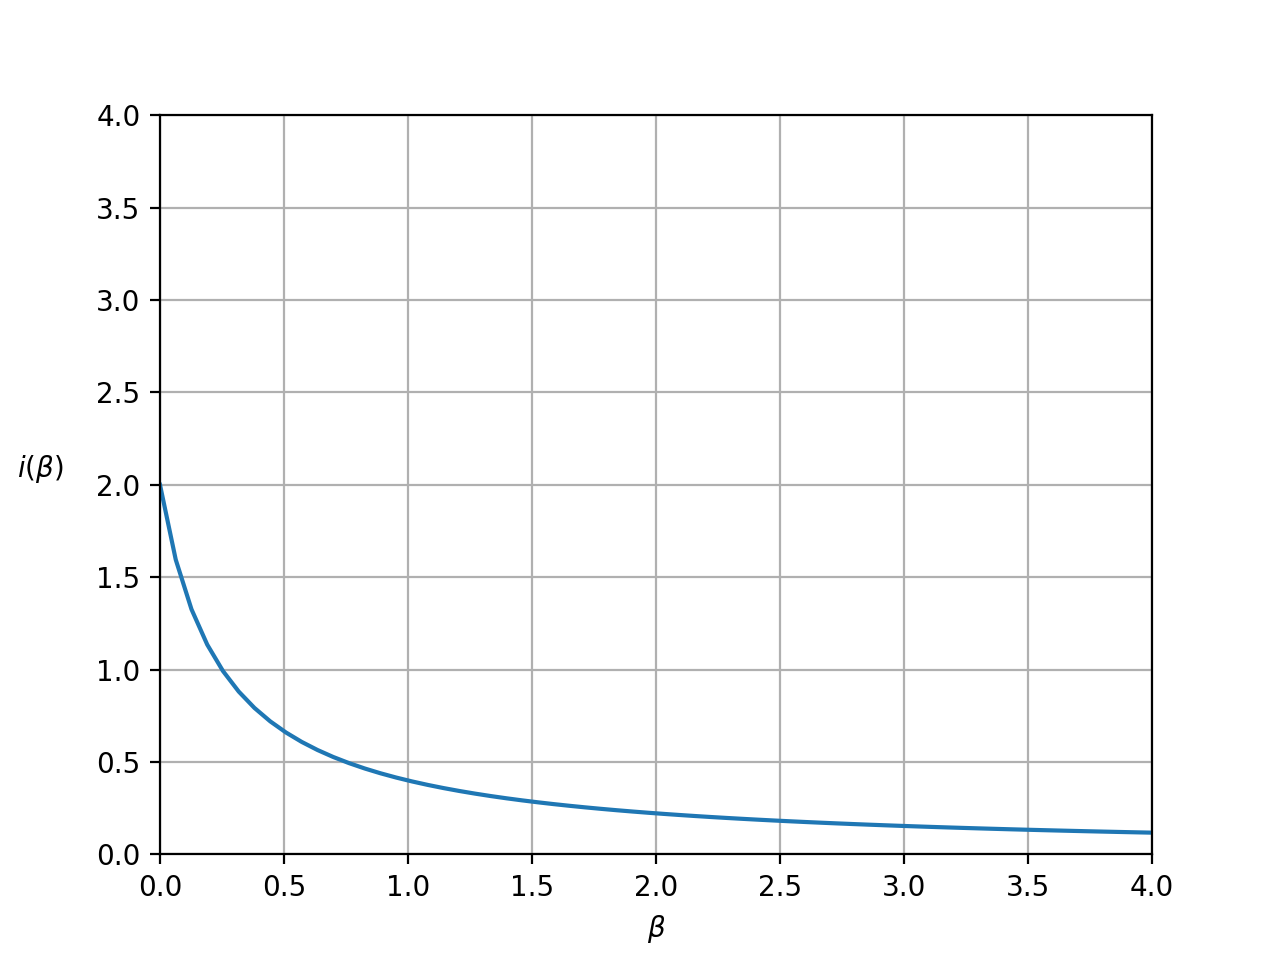
\includegraphics[width=11cm]{images/2010_2.png}
\end{figure}

分岐予測ミスをへらす技術的努力と結果得られる性能向上に関して、このグラフから言えることは分岐予測ミスを減らす技術的努力をすればするほど、分岐予測ミス削減による性能向上率も上がる。\\
グラフからは$\beta$が小さいほど、$\beta$を小さくしたときの$i(\beta)$の向上率が上がることが読み取れるからである。

\section*{第3問\ アルゴリズムとデータ構造}
\subsection*{(1)}

\subsection*{(2)}

\subsection*{(3)}

\subsection*{(4)}

\section*{第4問\ 情報通信}

\section*{第5問\ ネットワーク}
\subsection*{(1)}

\subsection*{(2)}

\subsection*{(3)}

\section*{第6問\ 信号処理}
\subsection*{(1)}

\subsection*{(2)}

\subsection*{(3)}

\subsection*{(4)}

\subsection*{(5)}

\end{document}

